%\documentclass{beamer} % use draft mode for speed !
\documentclass[aspectratio=1610]{beamer}
\usepackage{pacman}
\usepackage[english]{babel}
\usepackage[utf8]{inputenc}
\usepackage{amsmath, amsfonts, wasysym}
\usepackage{xcolor}
\usepackage{listings}
\usepackage{ulem}
\definecolor{darkgreen}{rgb}{.1,.7,.1}
\definecolor{darkred}{rgb}{.7,.1,.1}
\definecolor{darkblue}{rgb}{.1,.1,.7}
\lstset{language=python, basicstyle=\ttfamily,moredelim=[is][\textcolor{darkblue}]{@}{@},keywordstyle=\textcolor{darkblue},commentstyle=\textcolor{darkgreen},stringstyle=\textcolor{darkred},
        backgroundcolor=\color[gray]{0.9},
                frame=single
}

\usepackage{tikz}
\usetikzlibrary{positioning}
\usetikzlibrary{arrows}
\usetikzlibrary{calc}
\usetikzlibrary{backgrounds}
\usetikzlibrary{trees}
\usetikzlibrary{shadows}
\usetikzlibrary{positioning}
\usetikzlibrary{shadows}
\usetikzlibrary{arrows}
\usetikzlibrary{shapes}

\author[Serge Guelton, Pierrick Brunet, Mehdi Amini]{Serge Guelton \& Pierrick Brunet \& Mehdi Amini}

\title[\texttt{pythran}]{\texttt{Pythran} -- C++ for Snakes\\\emph{\small Static Compiler for High Performance}}

\date{\small{PyData - May 4th 2014}}

\institute{}

\begin{document}

\begin{frame}
  \maketitle
\vspace{-0.5cm}
  \begin{center}
    
\includegraphics[height=6em]{logo}
  \end{center}
  \vfill
  \hfill
  \scriptsize{Get the slides: http://goo.gl/6dgra0}
\end{frame}

% \begin{frame}[fragile]
%   \frametitle{Warning}
% 
% \begin{lstlisting}[language=python]
% from audience import you
% l=(Python, CXX, Compilation, Parallelism)
% skills=(x in you.__class__.__bases__
%     for x in l)
% if not any( skills ):
%     print("That's gonna be tough")
% \end{lstlisting}
% 
% \end{frame}

\begin{frame}[fragile]
    \frametitle{Disclaimer}

Timings were performed using OSX 10.9, an i7-3740QM CPU @ 2.70GHz, Python 2.7.6, current Pythran (branch Pydata2014), pypy 2.2.1, numba 0.13.1, gcc 4.8, Clang r207887.
\vfill
I am \textbf{not} Pythonista, but I'm interested in performance in general. 
\\ Daily job: driver-level C code, assembly, multi-threaded C++, GPU, ...
\vfill
\uncover<2->{
\begin{minipage}{0.4\textwidth}
\textit{Note: I love to troll, so let's have a beer later and talk
about how awful Python is! ;-)}
\end{minipage}
\hspace{0.09\textwidth}
\begin{minipage}{0.4\textwidth}
\uncover<3->{
    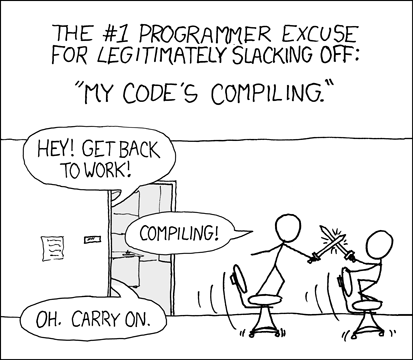
\includegraphics[width=0.9\textwidth]{compiling.png}
}
\end{minipage}
}
\vfill
\uncover<3->{
\scriptsize{
  By the way this talk is written in Latex and takes more than 10 seconds to
  \textbf{compile}.
}
}
\end{frame}


\begin{frame}{Prototyping Tools for Scientific Computing}
    \begin{tikzpicture}
        \node at (0,0) {
\includegraphics[height=4em]{matlab}};
        \only<1>{
            \node at (3,4) {
\includegraphics[height=4em]{python}};
        }
        \only<2>{
            \node[draw=darkblue, ultra thick,rounded corners] at (3,4) {
\includegraphics[height=4em]{python}};
        }
        \node at (9,3) {
\includegraphics[height=4em]{octave}};
        \node at (10,-1) {
\includegraphics[height=4em]{scilab}};
        \node at (6,2) {
\includegraphics[height=2em]{idl}};
    \end{tikzpicture}
\end{frame}

\begin{frame}{Tools for Scientific Computing in Python}
    \begin{tikzpicture}
        \node at (0,0) {
\includegraphics[height=4em]{pypy}};
        \node at (5,2) {
\includegraphics[height=4em]{numba}};
        \node at (10,5) {
\includegraphics[height=4em]{cython}};
        \node at (-1,6) {
\includegraphics[height=4em]{scipy_tool}};
        \node at (3,4.5) {
\includegraphics[height=2em]{theano}};
        \node at (.5,3) {\texttt{FORTRAN + f2py}};
        \node at (9.5,-.5) {\texttt{C + SWIG}};
    \end{tikzpicture}
\end{frame}

\begin{frame}{I Do not Know Much About Python But it Does not Matter Because...}

  \begin{center}
    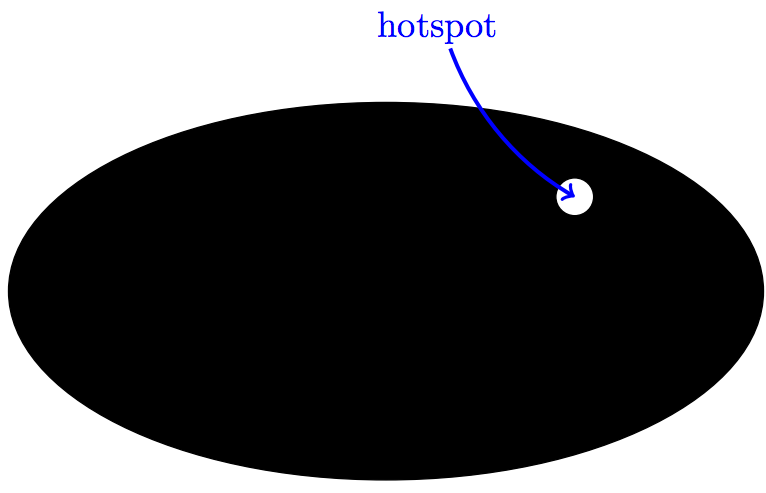
\includegraphics[width=0.6\textwidth]{hotspot}
  \end{center}
  
  I only care about the white spot.
\end{frame}


\begin{frame}[fragile]
    \frametitle{Regular IPython Session}
\begin{lstlisting}
>>> import numpy as np
>>> def rosen(x):
...    return sum(100.*(x[1:]-x[:-1]**2.)**2.
...         + (1-x[:-1])**2.)
>>> import numpy as np
>>> r = np.random.rand(100000)
>>> %timeit rosen(r)
10 loops, best of 3: @35.1 ms per loop@
\end{lstlisting}

\begin{quote}
In mathematical optimization, the Rosenbrock function is a non-convex function used as a performance test problem for optimization algorithms introduced by Howard H. Rosenbrock in 1960.[1] It is also known as Rosenbrock's valley or Rosenbrock's banana function. (Wikipedia)
\end{quote}

\end{frame}


\begin{frame}[fragile]
    \frametitle{IPython Session with Pythran}
\begin{lstlisting}
>>> %load_ext pythranmagic
>>> %%pythran
import numpy as np
#pythran export rosen(float[])
def rosen(x):
     return sum(100.*(x[1:]-x[:-1]**2.)**2.
        + (1-x[:-1])**2.)
>>> import numpy as np
>>> r = np.random.rand(100000)
>>> %timeit rosen(r)
10000 loops, best of 3: @121 us per loop@
\end{lstlisting}
\vfill
\uncover<2>{\centering{\Large That's a \alert{$\times$290} speedup!}}
\vfill

\end{frame}

\begin{frame}{Pythran's Meta Program Generator}
    \begin{center}
    \scalebox{1.1}{
    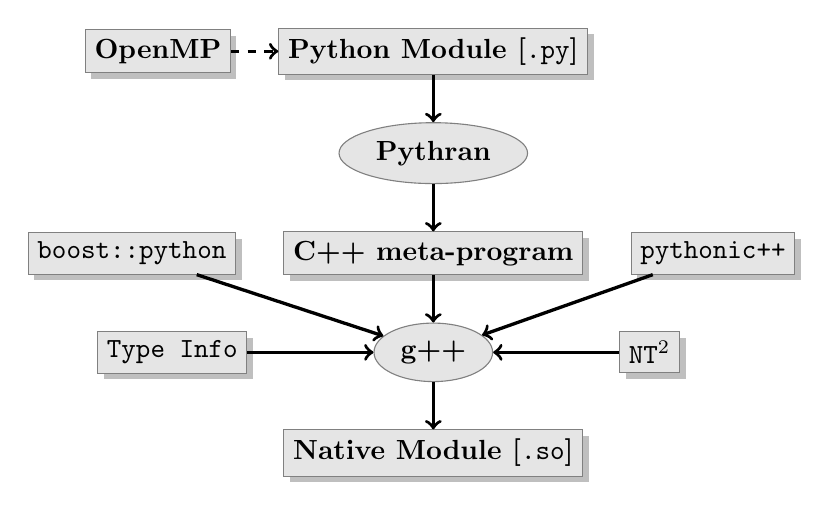
\begin{tikzpicture}[
            file/.style={draw=black!50,fill=black!10,rectangle, drop shadow, align=center,
            node distance=0.6cm},
                tool/.style={draw=black!50,fill=black!10,ellipse, align=center, node
            distance=0.6cm}]
            \node[file] (python) {\textbf{Python Module [\texttt{.py}]}};
            \node[file] (omp) [left=of python] {\textbf{OpenMP}};
            \node[tool] (pythran) [below=of python] {\textbf{Pythran}};
            \node[file] (cxx) [below=of pythran] {\textbf{C++ meta-program}};
            \node[file] (boost) [left=of cxx] {\textbf{\texttt{boost::python}}};
            \node[file] (pythonic) [right=of cxx] {\textbf{\texttt{pythonic++}}};
            \node[tool] (gxx) [below=of cxx] {\textbf{g++}};
            \node[file] (ti) [left=of gxx, xshift=-1cm] {\textbf{\texttt{Type Info}}};
            \node[file] (nt2) [right=of gxx, xshift=1cm] {\textbf{\texttt{NT}$^2$}};
            \node[file] (so) [below=of gxx] {\textbf{Native Module [\texttt{.so}]}};

            \draw[very thick, ->] (python) -- (pythran);
            \draw[very thick,dashed, ->] (omp) -- (python);
            \draw[very thick, ->] (pythran) -- (cxx);
            \draw[very thick, ->] (cxx) -- (gxx);
            \draw[very thick, ->] (boost) -- (gxx);
            \draw[very thick, ->] (pythonic) -- (gxx);
            \draw[very thick, ->] (ti) -- (gxx);
            \draw[very thick, ->] (nt2) -- (gxx);
            \draw[very thick, ->] (gxx) -- (so);
        \end{tikzpicture}
    }
\end{center}
\end{frame}

\begin{frame}{Pythran Moto}
    \begin{block}{Goals}
        \begin{enumerate}
                \centering{
                \item \structure{Performance First} \\\emph{sacrifice language feature}
                \item \structure{Subset of Python} \\\emph{backward compatibility matters} \\
                pythran $\approx$ python - useless stuff
                \\ \scriptsize\textit{(i.e. class, eval, introspection, polymorphic variable)} \normalsize
                \item \structure{Modular Compilation} \\\emph{focus on numerical kernels}
                }
        \end{enumerate}
    \end{block}

    \begin{block}{Means}
        \begin{enumerate}
                \centering{
                \item Static Compilation
                \item Static Optimizations
                \item Vectorization \& Parallelization
                }
        \end{enumerate}
    \end{block}
\end{frame}

\begin{frame}[fragile]
    \frametitle{A Story of Python \& C++}
    \begin{lstlisting}
def dot(l0, l1):
        return sum(x*y for x,y in zip(l0,l1))
        \end{lstlisting}
        \vspace{-1em}
        \begin{center}
            \Large$\simeq$
        \end{center}
        \vspace{-1em}
    \begin{lstlisting}[language=c++]
template<class T0, class T1>
auto dot(T0&& l0, T1&& l1)
-> decltype(/* ... */)
{
  return pythonic::sum(
    pythonic::map(
      operator_::multiply(),
        pythonic::zip(std::forward<T0>(l0),
                      std::forward<T1>(l1))
    ) );
}
        \end{lstlisting}
\end{frame}



\begin{frame}{C++ as a Back-end}
    \begin{block}{A High Level Language}
        \begin{itemize}
            \item Rich \structure{S}tandard \structure{T}emplate \structure{L}ibrary
            \item Object Oriented Programming
            \item Meta-Programming
            \item Glimpses of type inference\hfill\alert{\small C++11}
            \item Variadic Templates\hfill\alert{\small C++11}
        \end{itemize}
    \end{block}
    \begin{block}{A Low Level Language}
        \begin{itemize}
            \item Few Hidden Costs: "you don't pay for what you don't use"
            \item Direct access to vector instruction units \hfill\alert{SSE, AVX, \dots}
            \item Good for Parallel Programming \hfill\alert{OpenMP, TBB, \dots} \\ \hfill\scriptsize{(and the parallel STL is proposed for C++17)}
        \end{itemize}
    \end{block}
\end{frame}

\begin{frame}[fragile]
  \frametitle{Let's Dive Into the Backend Runtime... \uncover<2->{I'm Kidding!}}
    \begin{tikzpicture}
        \node at (0,0) {
  \begin{lstlisting}[language=c++,basicstyle=\ttfamily\scriptsize]
template <class Op, class S0, class... Iters>
  auto map_aux (Op &op, S0 const &seq, Iters... iters)
    -> sequence <decltype(op(*seq.begin(), *iters...))>
  {
    decltype(_map(op, seq, iters...)) s;
    auto iter = std::back_inserter(s);
    for(auto& iseq : seq)
      *iter ++= op(iseq , *iters++...);
    return s;
  }
template <class Op, class S0, class... SN>
  auto map ( Op op, S0 const &seq, SN const &... seqs )
    -> decltype(_map( op, seq, seqs.begin ()...)) 
  {
    return _map(op, seq, seqs.begin()...);
  }
\end{lstlisting}
        };
        \uncover<2->{
            \node at (6.5,0) {
                
\includegraphics[height=8em]{scream}
            };
        }
    \end{tikzpicture}
\end{frame}




\begin{frame}[fragile]
    \frametitle{Static Compilation}
    \begin{block}{Buys time for many time-consuming analyses}
        Points-to, used-def, variable scope, memory effects, function purity\dots
    \end{block}
    \begin{block}{Unleashes powerful C++ optimizations}
        Lazy Evaluation, Map Parallelizations, Constant Folding
    \end{block}
    \begin{block}{Requires static type inference}
        \begin{lstlisting}[lang=python]
        #pythran export foo(int list, float)
        \end{lstlisting}
        \centering Only annotate exported functions!
    \end{block}
\end{frame}

\begin{frame}{Pythran's Moto \textbf{1/3}}
\Large\centering Gather as many information as possible\\
\vfill
\normalsize(Typing is just one information among others)\\
\end{frame}


\begin{frame}[fragile]
    \frametitle{Example of Analysis: Points-to}
    \begin{lstlisting}[lang=python]
def foo(a,b):
    c = a or b
    return c*2
    \end{lstlisting}
    \vfill
    \centering\Large Where does \lstinline|c| points to ?
\end{frame}

\begin{frame}[fragile]
    \frametitle{Example of Analysis: Argument Effects}
    \begin{lstlisting}[lang=python]
def fib(n):
    return n if n<2 else fib(n-1) + fib(n-2)

def bar(l):
    return map(fib, l)

def foo(l):
    return map(fib, random.sample(l, 3))
    \end{lstlisting}
    \vfill
    \centering\Large Do \texttt{fibo}, \texttt{bar} and \texttt{foo} update their arguments?
\end{frame}

\begin{frame}[fragile]
    \frametitle{Example of Analysis: Pure Functions}
    \begin{lstlisting}[lang=python]
def f0(a):
    return a**2

def f1(a):
    b = f0(a)
    print b
    return b

l = list(...)
map(f0, l)
map(f1, l)
    \end{lstlisting}
    \vfill\centering\Large Are \texttt{f0} and \texttt{f1} pure functions?
\end{frame}

\begin{frame}[fragile]
    \frametitle{Example of Analysis: Use - Def Chains}
    \begin{lstlisting}[lang=python]
a = '1'
if cond:
    a = int(a)
else:
    a = 3
print a
a = 4
    \end{lstlisting}
    \vfill\centering\Large Which version of \texttt{a} is seen by the \texttt{print} statement?
\end{frame}

\begin{frame}{Pythran's Moto \textbf{2/3}}
    \begin{center}
        Gather as many information as possible\\
        \vfill
        \Large Turn them into Code Optimizations!
        \vfill
    \end{center}
\end{frame}


\begin{frame}[fragile]
    \frametitle{Example of Code Optimization: False Polymorphism}
    \begin{lstlisting}
a = cos(1)
if cond:
    a = str(a)
else:
    a = None
foo(a)
\end{lstlisting}
\vfill\centering\Large Is this code snippet statically typable?
\end{frame}

\begin{frame}[fragile]
    \frametitle{Example of Code Optimization: Lazy Iterators}
    \begin{lstlisting}
def valid_conversion(n):
    l = map(math.cos, range(n))
    return sum(l)

def invalid_conversion(n):
    l = map(math.cos, range(n))
    l[0] = 1
    return sum(l) + max(l)
    \end{lstlisting}
    \vfill\centering\Large Which \texttt{map} can be converted into an \texttt{imap}
\end{frame}

\begin{frame}[fragile]
    \frametitle{Example of Code Optimization: Constant Folding}
    \begin{lstlisting}[lang=python]
def esieve(n):
    candidates = range(2, n+1)
    return sorted(
        set(candidates) - set(p*i
                              for p in candidates
                              for i in range(p, n+1))
        )

cache = esieve(100)
    \end{lstlisting}
    \vfill\centering\Large Can we evalute \texttt{esieve} at compile time?

\end{frame}

\begin{frame}{Pythran's Moto \textbf{3/3}}
    \begin{center}
Gather as many information as possible\\
\vfill
Turn them into Code Optimizations\\
\vfill
\Large Vectorize! Parallelize!
\end{center}
\end{frame}

\begin{frame}[fragile]
    \frametitle{Explicit Parallelization}
            \begin{lstlisting}[basicstyle=\ttfamily\scriptsize]
def hyantes(xmin, ymin, xmax, ymax, step, range_, range_x, range_y, t):
  pt = [[0]*range_y for _ in range(range_x)]
  #omp parallel for
  for i in xrange(range_x):
    for j in xrange(range_y):
      s = 0
      for k in t:
        tmp = 6368.* math.acos(math.cos(xmin+step*i)*math.cos( k[0] ) *
                               math.cos((ymin+step*j)-k[1]) +
                               math.sin(xmin+step*i)*math.sin(k[0]))
        if tmp < range_:
          s+=k[2] / (1+tmp)
      pt[i][j] = s
  return pt
\end{lstlisting}
\vfill
    \begin{tabular}{|l|r|r|r|}
        \hline
     Tool    &  CPython    &   Pythran     & OpenMP   \\
    \hline
     Timing  &  639.0ms    &   44.8ms       &      11.2ms       \\
    \hline
     Speedup &  $\times$1         &    $\times$14.2      &    $\times$57.7   \\
    \hline
\end{tabular}
\end{frame}

\begin{frame}{Library Level Optimizations}
    \begin{block}{Numpy is the \structure{key}}
        \begin{itemize}
            \item Basic block of Python Scientific Computing
            \item High-level Array Manipulations
            \item Many common functions implemented
        \end{itemize}
    \end{block}
    \begin{enumerate}
        \item This smells like FORTRAN
        \item For the compiler guy, FORTRAN smells good
        \item Unlock vectorization \& parallelization of Numpy code!
    \end{enumerate}
    
    \vfill
    \begin{center}
    \scriptsize{Cython is known to be "as fast as C", the only way we found to beat it is to be "as fast as Fortran", hence: Py\textbf{thran}}
    \end{center}
    
\end{frame}

\begin{frame}{Efficient Numpy Expressions}
    \begin{block}{Expression Templates}
        \begin{enumerate}
            \item A classic C++ meta-programming optimization
            \item Brings Lazy Evaluation to C++
            \item Equivalent to loop fusion
        \end{enumerate}
    \end{block}

    \begin{block}{More Optimizations}
        \begin{itemize}
            \item vectorization through \texttt{boost::simd} and \texttt{nt2}
            \item parallelization through \texttt{\#pragma omp}
        \end{itemize}
    \end{block}
\end{frame}


% \begin{frame}[fragile]
%     \frametitle{Benchmark}
%     \begin{lstlisting}
% def arc_dist(theta_1, phi_1, theta_2, phi_2):
%     temp = (np.sin((theta_2-theta_1)/2)**2
%         + np.cos(theta_1)*np.cos(theta_2)
%         * np.sin((phi_2-phi_1)/2)**2)
%     distance_matrix = 2 * np.arctan2(
%             sqrt(temp),sqrt(1-temp))
%     return distance_matrix
%     \end{lstlisting}
% 
%     \vfill
% 
%     \begin{tabular}{|l|r|r|r|r|}
%         \hline
%         Tool    &  CPython    &  Cython  &  Numexpr    & Pythran   \\
%         \hline
%         Timing  &  192.2ms    &  36.0ms  &    41.2ms   &  17.1ms   \\
%         \hline
%         Speedup &  $\times$1         &  $\times$5.33   &  $\times$4.67      &  $\times$11.23   \\
%         \hline
%     \end{tabular}
% \end{frame}

\begin{frame}[fragile]
    \frametitle{Julia Set, a Cython Example}

\begin{lstlisting}
def run_julia(cr, ci, N, bound, lim, cutoff):
    julia = np.empty((N, N), np.uint32)
    grid_x = np.linspace(-bound, bound, N)
    t0 = time()
    #omp parallel for
    for i, x in enumerate(grid_x):
        for j, y in enumerate(grid_x):
            julia[i,j] = kernel(x, y, cr, ci, lim, cutoff)
    return julia, time() - t0
\end{lstlisting}
From Scipy2013 Cython Tutorial.
\vfill
    \begin{tabular}{|l|r|r|r|r|}
        \hline
        Tool    &  CPython    &  Cython  &  Pythran & +OpenMP   \\
        \hline
        Timing  &  3630ms    &   4.3ms  &   3.71ms  & 1.52ms  \\
        \hline
        Speedup & $\times$1 &  $\times$837 &  $\times$970 & $\times$2368   \\
        \hline
    \end{tabular}

\end{frame}


\begin{frame}[fragile]
    \frametitle{Mandelbrot, a Numba example}
    \begin{minipage}{0.49\textwidth}
\begin{lstlisting}[language=Python,frame=none,backgroundcolor=\color{white},basicstyle=\ttfamily\tiny]
@autojit
def mandel(x, y, max_iters):
    """
    Given the real and imaginary parts of a complex number,
    determine if it is a candidate for membership in the Mandelbrot
    set given a fixed number of iterations.
    """
    i = 0
    c = complex(x, y)
    z = 0.0j
    for i in range(max_iters):
        z = z**2 + c
        if abs(z)**2 >= 4:
            return i

    return 255
    \end{lstlisting}
\end{minipage}
\begin{minipage}{0.49\textwidth} \begin{lstlisting}[language=Python,frame=none,backgroundcolor=\color{white},basicstyle=\ttfamily\tiny]
@autojit
def create_fractal(min_x, max_x, min_y, max_y, image, iters):
    height = image.shape[0]
    width = image.shape[1]

    pixel_size_x = (max_x - min_x) / width
    pixel_size_y = (max_y - min_y) / height
    
    for x in range(width):
        real = min_x + x * pixel_size_x
        for y in range(height):
            imag = min_y + y * pixel_size_y
            color = mandel(real, imag, iters)
            image[y, x] = color

    return image
\end{lstlisting}
\end{minipage}
    \vfill
    \begin{tabular}{|l|r|r|r|r|}
        \hline
     Tool    &  CPython    &   Numba    &   Pythran  \\
        \hline
     Timing  &  8170ms   &    56ms       &   47.2ms  \\
        \hline
     Speedup & $\times$1 & $\times$145 & $\times$173 \\
    \hline
\end{tabular}

\scriptsize{"g++ -Ofast" here}
\end{frame}

\begin{frame}[fragile]
    \frametitle{Nqueens, to Show Some Cool Python}
    \begin{minipage}{0.49\textwidth}
            \begin{lstlisting}[frame=none,backgroundcolor=\color{white},basicstyle=\ttfamily\tiny]
# Pure-Python implementation of
# itertools.permutations()
# Why? Because we can :-)
def permutations(iterable, r=None):
  pool = tuple(iterable)
  n = len(pool)
  if r is None:
    r = n
  indices = range(n)
  cycles = range(n-r+1, n+1)[::-1]
  yield tuple(pool[i] for i in indices[:r])
  while n:
    for i in reversed(xrange(r)):
      cycles[i] -= 1
      if cycles[i] == 0:
        indices[i:] = indices[i+1:] + indices[i:i+1]
        cycles[i] = n - i
      else:
        j = cycles[i]
        indices[i], indices[-j] = \
            indices[-j], indices[i]
        yield tuple(pool[i] for i in indices[:r])
        break
    else:
      return
    \end{lstlisting}
\end{minipage}
\begin{minipage}{0.49\textwidth}
            \begin{lstlisting}[frame=none,backgroundcolor=\color{white},basicstyle=\ttfamily\tiny]
#pythran export n_queens(int)
def n_queens(queen_count):
  """N-Queens solver.
  Args:
    queen_count: the number of queens to solve
    for. This is also the board size.

  Yields:
    Solutions to the problem. Each yielded 
    value is looks like (3, 8, 2, ..., 6) 
    where each number is the column position 
    for the queen, and the index into the 
    tuple indicates the row.
  """
  out =list()
  cols = range(queen_count)
  for vec in permutations(cols,None):
    if (queen_count == len(set(vec[i]+i 
                               for i in cols))):
      out.append(vec)
  return out
\end{lstlisting}
\end{minipage}

    \begin{minipage}{0.49\textwidth}
      \scriptsize
Solving the NQueen problem, using generator, generator expression, list comprehension, sets\dots
    \\ http://code.google.com/p/unladen-swallow/
    \normalsize
\end{minipage}
\begin{minipage}{0.49\textwidth}

    \begin{tabular}{|l|r|r|r|r|}
        \hline
     Tool    &  CPython    &     PyPy     &  Pythran  \\
        \hline
     Timing  &  2640.6ms   &    501.1ms   &  693.3ms  \\
        \hline
     Speedup & $\times$1   & $\times$5.27 & $\times$3.8 \\
    \hline
\end{tabular}
\end{minipage}

\end{frame}




\begin{frame}[fragile]
    \frametitle{Numpy Benchmarks}
   
   \resizebox {\textwidth} {!} {
    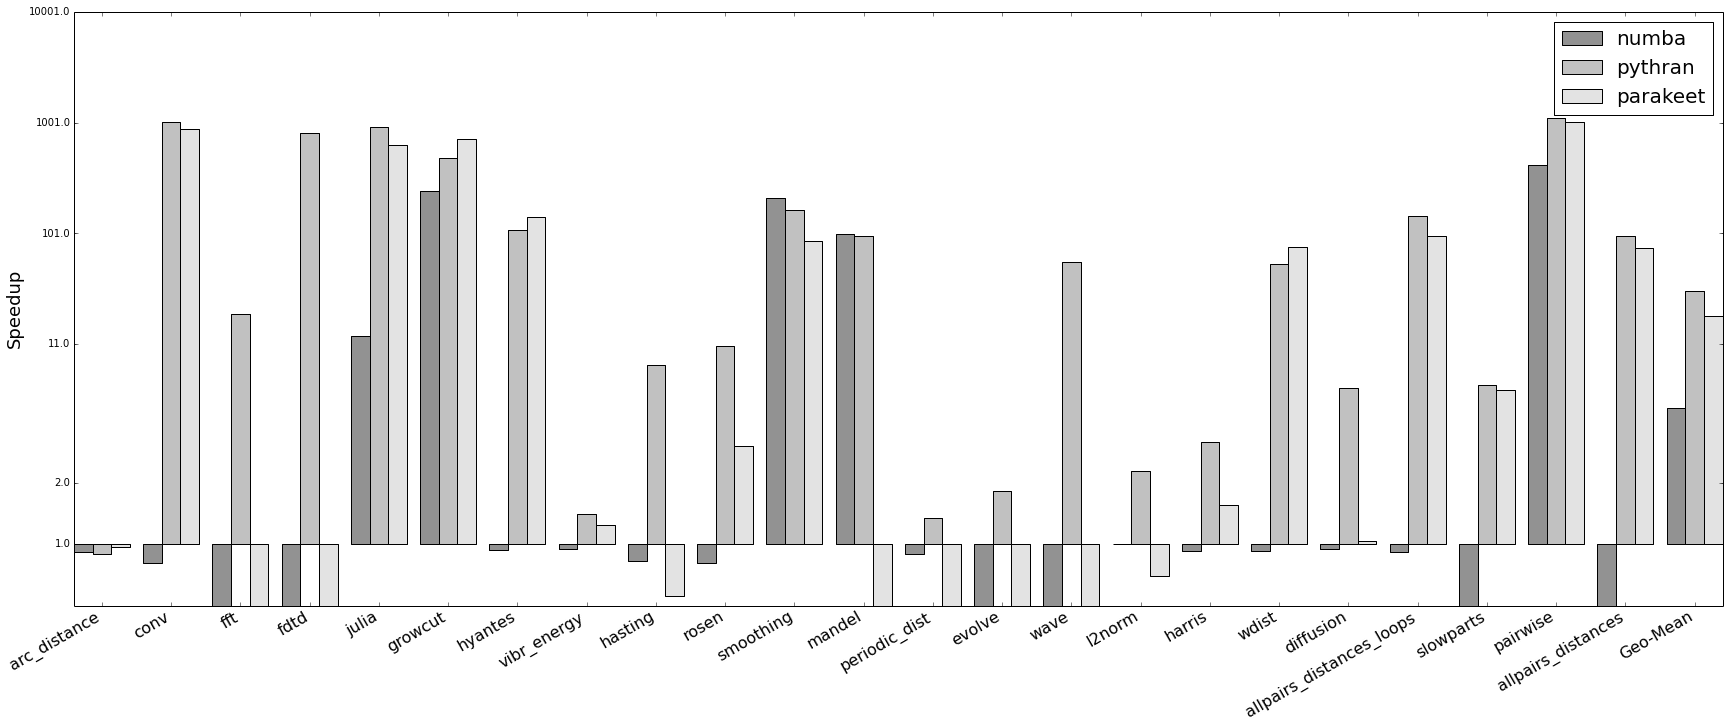
\includegraphics{timing}
   }
    \url{https://github.com/serge-sans-paille/numpy-benchmarks/}

\vfill
    \scriptsize{Made with Matplotlib last night!}
\vfill
   
    \tiny{Debian clang version 3.5-1~exp1, x86-64, i7-3520M CPU @ 2.90GHz. No OpenMP/Vectorization for Pythran.}
\end{frame}


\begin{frame}{Crushing the Head of the Snake}

  \begin{center}
    
\includegraphics[width=0.8\textwidth]{crushing}

\vfill
  I would have titled it "What every Pythonista should know about Python!"
\vfill
  
  \tiny (hopefully we'll get the video soon).
\vfill
  \end{center}

\end{frame}


\begin{frame}[fragile]
  \frametitle{The Compiler Is not the Solution to Keyboard-Chair Interface, Is It?}
    \begin{minipage}{0.49\textwidth}
\begin{lstlisting}[language=Python,frame=none,backgroundcolor=\color{white},basicstyle=\ttfamily\tiny]
def total(arr):
    s = 0
    for j in range(len(arr)):
        s += arr[j]
    return s


def varsum(arr):
    vs = 0
    for j in range(len(arr)):
        mean = (total(arr) / len(arr))
        vs += (arr[j] - mean) ** 2
    return vs
    
\end{lstlisting}
\end{minipage}
\begin{minipage}{0.49\textwidth} \begin{lstlisting}[language=Python,frame=none,backgroundcolor=\color{white},basicstyle=\ttfamily\tiny]
#pythran export stddev(float64 list list)
def stddev(partitions):
    ddof=1
    final = 0.0
    for part in partitions:
        m = total(part) / len(part)
        # Find the mean of the entire grup.
        gtotal = total([total(p) for p in partitions])
        glength = total([len(p) for p in partitions])
        g = gtotal / glength
        adj = ((2 * total(part) * (m - g)) + ((g ** 2 - m ** 2) * len(part)))
        final += varsum(part) + adj
    return math.sqrt(final / (glength - ddof))
\end{lstlisting}
\end{minipage}
\vfill
\begin{tabular}{|l|r|r|r|r|r|r|}
  \hline
  Version  &  Awful     &  Less Awful  &  OK & \textit{Differently OK} & \textit{OK} & Numpy   \\
  \hline
  CPython  & 127s       &   150ms  &   54.3ms  & 53.8ms    & 47.6ms & 8.2ms  \\
  \hline
  
  Pythran  & \uncover<2-> {1.38s}      &   \uncover<3-> {4.7ms}  &   \uncover<4-> {4.8ms}   &  \uncover<5-> {5.8ms}    &  \uncover<6-> {4.7ms} & \uncover<7-> {1.7ms} \\
        \hline
    \end{tabular}

\end{frame}


\begin{frame}{Engineering Stuff}
    \begin{block}{Get It}
        \begin{itemize}
            \item Follow the source: \url{https://github.com/serge-sans-paille/pythran} \\ \textit{(we are waiting for your pull requests)}
            \item Debian repo: \texttt{deb http://ridee.enstb.org/debian unstable main}
            \item Join us: \texttt{\#pythran} on Freenode 
            \textit{(very active)}, \\ or \url{pythran@freelists.org} 
            \textit{(not very active)}
        \end{itemize}
    \end{block}

    Available on PyPI, using Python 2.7, +2000 test cases, PEP8 approved, clang++ \& g++ ($>=4.8$) friendly, Linux and OSX validated.
\end{frame}

\begin{frame}[fragile]{Conclusion}
    \normalsize
        \vfill
        Compiling Python means more than typing and translating\\
        \vfill
        \uncover<2-> {
        \vfill
        What next: 
        \vfill
        \begin{itemize}
          \item<2-> Release the PyData version  
          \only<3>{\scriptsize{(ooops we're late)}} \only<4-> {\scriptsize{(\sout{ooops we're late} I did not specify which year)}}
          \item<4-> User module import \scriptsize{(pull request already issued)}
          \item<5-> Set-up an daily performance regression test bot \scriptsize{(ongoing work with codespeed)}
          \item<6-> Re-enable vectorization through boost::simd and nt2 \scriptsize{(soon)}
          \item<7-> More Numpy support, start looking into Scipy
          \item<8-> Polyhedral transformations \scriptsize{(in another life...)}
        \end{itemize}
        }
        \vfill
        % \uncover<3->{
        %     Need a compiler guy / HPC Engineer? I am looking for a job!\\
        % }
        \vfill
    \hfill\tiny{\url{http://pythonhosted.org/pythran/}}
\end{frame}




\end{document}
% vim:spell spelllang=fr
